%% horizontal_self_org.tex
In this thesis, two different concepts of self-organisation are implemented.
This chapter presents a method based on horizontal self-organisation.
Horizontal self-organisation is based on training small units within a network independent from each other.
The first section presents the methodology (i.e. how it is implemented), and the second section evaluates the models and analyses the obtained results.


\section{Methods}\seclbl{horizontal_self_org_methods}
The first choice for networks based on horizontal self-organisation is what the independent units are, i.e. which group of network parameters are trained independently.
In this thesis, a single layer is used as a self-contained unit. A layer is a small unit (e.g. compared to a model part that contains many layers) but can still be trained efficiently.
Smaller units would be neurons or parts of a layer, but training them separately would be slow since the efficiency of matrix operations on GPUs could no longer be fully exploited.

Each layer optimises a proxy objective function.
Proxy objective functions are used because this type of local optimisation allows self-organisation and excellent performance on larger datasets \sidecite{Bartunov_Santoro_Richards_Marris_Hinton_Lillicrap_2018, Duan_Principe_2022}, in contrast to other local learning algorithms such as target propagation, synthetic gradients or feedback alignment (c.f. \secref{alt_train_algo}). 
 \figref{horizontal_gradient_flow} visualises the updates based on proxy objective functions.
An objective function is calculated for each layer, and the optimisation algorithm only updates the parameters within this layer.
Thus, the gradients do not flow back to the preceding layers.

\begin{figure}[h]
    \centering
    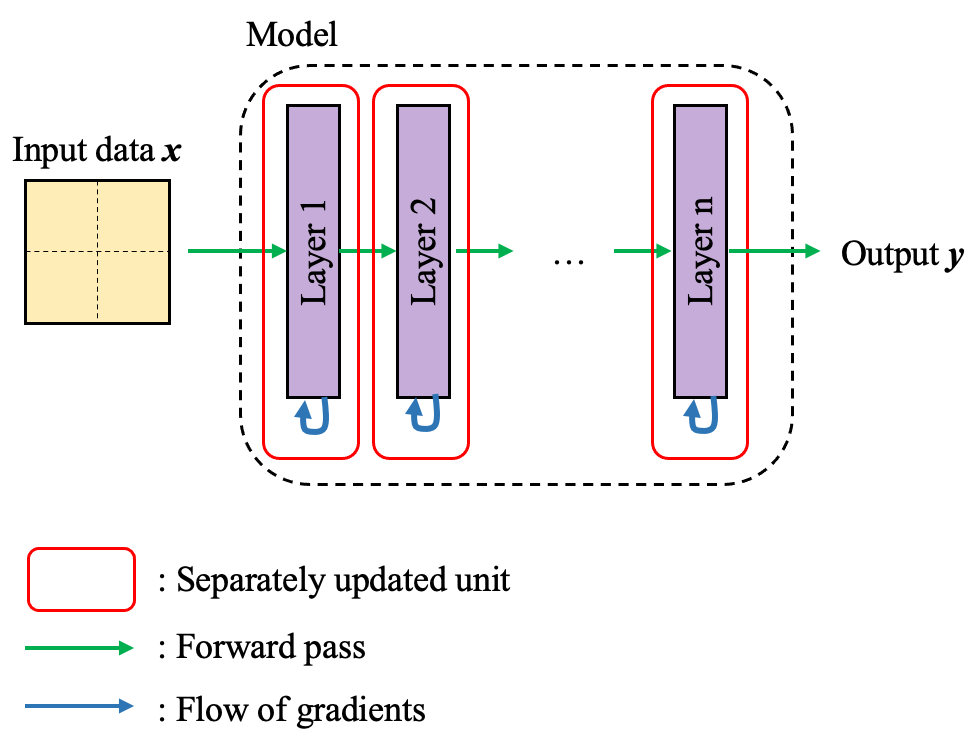
\includegraphics[width=0.89\textwidth]{horizontal_gradient_flow}
    \caption[The flow of gradients within the network based on horizontal self-organisation]{The flow of gradients within the network based on horizontal self-organisation: The data is fed from layer to layer during the forward pass. The layers are trained independently, and the gradients do not flow backwards to the previous layers.}
    \figlbl{horizontal_gradient_flow}
\end{figure}

A combination of diversity and sparsity constraints is used as a loss function, which leads to representations that are easy to interpret, suitable for net fragments (c.f. \secref{neuro_concepts_net_fragments}), and also increases robustness (c.f. \secref{neuro_concepts_sparsity}).
Identical to the preliminary experiments in Appendix \chref*{net_fragments}, the sparsity is achieved by using the kullback-leibler (KL) divergence \sidecite{10-5555-3042573-3042641}.

The model consists of several linear layers $l$ with a ReLU activation function (c.f. \eqref{act_functions}).
A layer $l$ consists of $n^{[l]}$ neurons and the activations $\boldsymbol{a}^{[l]}$ are calculated for a given input $\boldsymbol{a}^{[l-1]}$ as

\begin{align}\eqlbl{vso_1}
		\boldsymbol{a}^{[l]} = f \left( \boldsymbol{W}^{[l]} \cdot \boldsymbol{a}^{([l-1]} + \boldsymbol{b}^{[l]} \right)
\end{align}

whereby $\boldsymbol{W}^{[l]}$ is the weight, $\boldsymbol{b}^{[l]}$ the bias of layer $l$, and $f(\cdot)$ is the activation function.
If a mini-batch contains $m$ samples, the activation probability $\hat{\rho}^{[l]}_i$ of a neuron $a^{[l]}_i$ can be calculated as:

\begin{align}\eqlbl{vso_2}
		\hat{\rho}^{[l]}_i= \frac{1}{m} \sum^m_{i=1} \left( \frac{1}{1+e^{-a^{[l]}_i}} \right)
\end{align}

where $\left( \frac{1}{1+e^{-a^{[l]}_i}} \right)$ is the sigmoid function that squeezes the activation in the range between $0$ and $1$.
With the KL divergence, the divergence of the actual activation probability $\hat{\rho}^{[l]}_i$ and a desired activation probability $\rho=0.05$ can be calculated:

\begin{align}\eqlbl{vso_3}
		KL(\rho || \hat{\rho}^{[l]}_i) = \rho \cdot \log \frac{\rho}{\hat{\rho}^{[l]}_i} + (1-\rho) \cdot \log \frac{1-\rho}{1-\hat{\rho}^{[l]}_i}
\end{align}

The sparsity loss $\mathcal{L}^{[l]}_{s}$ of layer $l$ is the sum of the divergence between each neuron's activation probability $\hat{\rho}^{[l]}_i$ and the target activation probability $\rho$:

\begin{align}\eqlbl{vso_4}
		\mathcal{L}^{[l]}_{s} = \sum_{i=1}^{n} KL(\rho || \hat{\rho}^{[l]}_i)
\end{align}

Thus, it is enforced that $5\%$ of the neurons are active per sample.
The second constraint is a diversity constraint. The goal is that the activations of \emph{different} objects are diverse. For this purpose, the activations $\boldsymbol{a}^{[l]}$ are made as identical as possible (i.e. pushed together in feature space) if they stem from the same class and as different as possible if they stem from different classes.
The cosine similarity is used to calculate the similarity between the activations $\boldsymbol{a}^{[l](i)}$ and $\boldsymbol{a}^{[l](j)}$ of two samples $\boldsymbol{x}^{(i)}$ and $\boldsymbol{x}^{(j)}$:

\begin{align}\eqlbl{vso_5}
		\text{cos}\left( \boldsymbol{a}^{[l](i)}, \boldsymbol{a}^{[l](j)} \right) = \frac{\boldsymbol{a}^{[l](i)} \cdot \boldsymbol{a}^{[l](j)}}{\max \left( ||\boldsymbol{a}^{[l](i)}||_2, ||\boldsymbol{a}^{[l](j)}||_2 \right)}
\end{align}

The information of image labels $y^{(i)} \in C$ is needed to push representations of identical objects together or to push representations of different objects apart.
The diversity loss $\mathcal{L}^{[l]}_d$ minimises the cosine similarity if the activations stem from different classes (i.e. $y^{(i)} \neq y^{(j)}$), or maximises the similarity if they stem from the same class (i.e. $y^{(i)} = y^{(j)}$).

\begin{align}\eqlbl{vso_6}
		\mathcal{L}^{[l]}_{d} = \frac{1}{n^2} \sum_{i=1}^{n} \sum_{j=1}^{n} k \cdot \text{cos} \left( \boldsymbol{a}^{[l](i)}, \boldsymbol{a}^{[l](j)} \right) \text{ if } i \neq j
\end{align}

whereby $k$ changes the sign depending on the class:

\begin{align}\eqlbl{vso_7}
		k = \begin{cases}
      		+1, & \text{if}\ y^{(i)} \neq y^{(j)} \\
      		-1, & \text{otherwise}
    	\end{cases}
\end{align}


However, this loss function has two significant drawbacks: First, comparing two samples can be unstable; if one sample is not representative of a class, the other sample may be pushed away from its classes' cluster centre. Second, if the dataset has more than two classes, more negative samples ( $y^{(i)} \neq y^{(j)}$) than positive samples ($y^{(i)} = y^{(j)}$) are compared. With many classes, the optimisation algorithm focuses mainly on pushing negative samples apart and does not pay enough attention to pushing positive samples together. These problems are alleviated with two measures: Instead of comparing two samples, a sample is compared to the average activation of a class, which can be interpreted as the cluster centre of a class. Furthermore, each sample is once compared with the cluster centre from the same class and once with a cluster centre from another class. Thus, positive and negative samples are compared equally often.

Lets denote {\footnotesize $\boldsymbol{a}^{[l]}_{C=\overline{c}}$} as the average activation of class $c$ in layer $l$. Thus, the goal is to push the activation of a sample $\boldsymbol{a}^{[l](i)}$ closer to {\footnotesize $\boldsymbol{a}^{[l]}_{C=\overline{y}^{(i)}}$} and away from {\footnotesize $\boldsymbol{a}^{[l]}_{C=\overline{v}^{(i)}}$}, where $v^{(i)}$ is a random class drawn from $ C \backslash \{y^{(i)} \}$\sidenote{the set of all classes without $y^{(i)}$}. Such a loss could be implemented as

\begin{align}\eqlbl{vso_8}
		\mathcal{L}^{[l]}_{d}  = \frac{1}{n} \sum_{i=1}^{n} \text{cos} \left(\boldsymbol{a}^{[l](i)}, \boldsymbol{a}^{[l]}_{C=\overline{v}^{(i)}} \right) - \text{cos} \left(\boldsymbol{a}^{[l](i)}, \boldsymbol{a}^{[l]}_{C=\overline{y}^{(i)}} \right)
\end{align}

However, the problem with this loss is that all cosine similarities become $1$, and the loss becomes $0$ if all activations are identical.
Therefore, a margin between the similarities is enforced, similar to the triplet-margin-loss  \sidecite{Balntas_Riba_Ponsa_Mikolajczyk_2016}.


\begin{align}\eqlbl{vso_9}
\begin{split}
		\mathcal{L}^{[l]}_{d} = \frac{1}{n} \sum_{i=1}^{n} \max \biggl[ & \text{cos} \left(\boldsymbol{a}^{[l](i)}, \boldsymbol{a}^{[l]}_{C=\overline{v}^{(i)}} \right) \\
		& - \text{cos} \left(\boldsymbol{a}^{[l](i)}, \boldsymbol{a}^{[l]}_{C=\overline{y}^{(i)}} \right) + \text{margin}, 1 \biggr]
\end{split}
\end{align}

where $\text{margin}$ is a hpyerparameter that is set to $1$.
The loss applied to each layer is the sum of sparsity loss and diversity loss, with the diversity loss weighted by $\lambda=0.1$:
\begin{align}\eqlbl{vso_10}
		\mathcal{L}^{[l]} =\mathcal{L}^{[l]}_{s} + \lambda \cdot \mathcal{L}^{[l]}_{d}
\end{align}


One problem with proxy objective functions is that this type of training often requires layer-wise training. I.e. first layer $1$ is trained until convergence, then the weights are frozen, afterwards layer $2$ is trained and so on.
Such sequential training is inefficient because it requires more forward passes than if the model is trained with end-to-end backpropagation.
It was found that the proposed loss function allows training all layers simultaneously. With a forward pass, all activations are calculated, followed by a layer-wise backward pass where the gradients from one layer do not propagate back to previous layers.
Since the gradients are only needed locally, no large graph of gradients has to be calculated, which reduces the memory utilisation on GPUs and allows larger mini-batch sizes. In addition, this type of architecture is straightforward to parallelise since each layer (i.e. each independently trained unit) or a group of layers can be trained on a different GPU:

\begin{figure}[h]
    \centering
    \resizebox{0.99\textwidth}{!}
{
\begin{tikzpicture}
\tikzstyle{connection}=[ultra thick,every node/.style={sloped,allow upside down},draw=\edgecolor,opacity=0.7]
\tikzstyle{copyconnection}=[ultra thick,every node/.style={sloped,allow upside down},draw={rgb:blue,4;red,1;green,1;black,3},opacity=0.7]


\node[canvas is zy plane at x=0] (input) at (0,0,0) {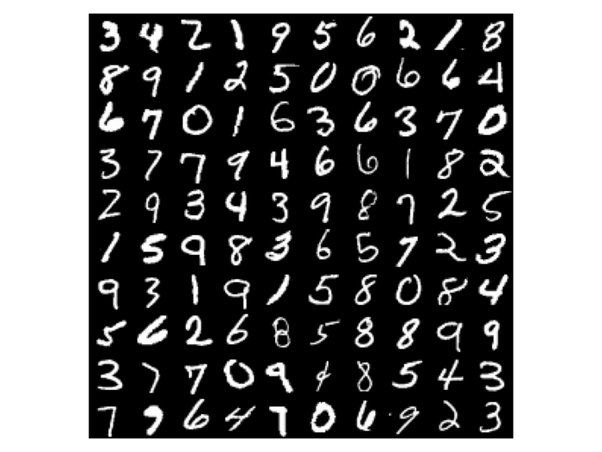
\includegraphics[width=8cm,height=8cm]{imgs/mnist.jpeg}};


\pic[shift={(3,0,0)}] at (input) 
    {Box={
        name=fcn1,
        caption=FC + ReLU,
        xlabel={{" ","dummy"}},
        zlabel=512,
        fill=\SoftmaxColor,
        opacity=0.8,
        height=3,
        width=3,
        depth=52
        }
    };


\draw [connection]  (input) ++(0,0,0)    -- node {\midarrow} (fcn1-west);


\pic[shift={(2,0,0)}] at (fcn1-east) 
    {Box={
        name=fcn2,
        caption=FC + ReLU,
        xlabel={{" ","dummy"}},
        zlabel=256,
        fill=\SoftmaxColor,
        opacity=0.8,
        height=3,
        width=3,
        depth=25
        }
    };


\draw [connection]  (fcn1-east)    -- node {\midarrow} (fcn2-west);


\pic[shift={(2,0,0)}] at (fcn2-east) 
    {Box={
        name=fcn3,
        caption=FC + ReLU,
        xlabel={{" ","dummy"}},
        zlabel=128,
        fill=\SoftmaxColor,
        opacity=0.8,
        height=3,
        width=3,
        depth=13
        }
    };


\draw [connection]  (fcn2-east)    -- node {\midarrow} (fcn3-west);


\pic[shift={(2,0,0)}] at (fcn3-east) 
    {Box={
        name=fcn4,
        caption=FC + ReLU,
        xlabel={{" ","dummy"}},
        zlabel=64,
        fill=\SoftmaxColor,
        opacity=0.8,
        height=3,
        width=3,
        depth=6
        }
    };


\draw [connection]  (fcn3-east)    -- node {\midarrow} (fcn4-west);


\end{tikzpicture}
}
    \caption[Architecture of the fully connected model with horizontal self-organisation]{The network architecture of the fully connected model for horizontal self-organisation with fully connected layers.}
    \figlbl{horizontal_org_arch1}
\end{figure}

The model used in this thesis consists of $4$ fully connected layers with ReLU activation. The first layer has $512$ neurons, the second $256$ neurons, the third $128$ neurons and the fourth $64$ neurons. The model is illustrated in \figref{horizontal_org_arch1}. Each layer is trained separately by minimising the loss  $\mathcal{L}^{[l]}$ (c.f. \eqref{vso_10}) with the Adam optimizer \sidecite{Kingma2015AdamAM} and a learning rate of $\eta = 1 \cdot 10^{-3}$. The mini-batch size is $60,000$. 

\subsection{Extraction of Representations}\seclbl{horizontal_self_org_representations}
In accordance with net fragments as defined in \secref{neuro_concepts_net_fragments}, the representations are not extracted at a specific point in the network (i.e. a pre-defined layer), but all representations from all layers are taken into account to fulfil a task.
In the following, this is demonstrated based on a classification task, but other tasks are also conceivable in the future.
After training, the average activation {\footnotesize $\boldsymbol{a}^{[l]}_{C=\overline{c}}$} for each class $c \in C$ and layer $l$ is calculated.
These averages from the training set represent prototypes of each class in each layer and can be considered a reference representation per class. Thus, the representations needed for this task are computed \emph{after} training and are not part of the training as, for example, in the case of a classification loss based on cross-entropy.
When a new sample $\boldsymbol{x}^{(i)}$ is classified, the cosine similarity between the activations {\footnotesize $\boldsymbol{a}^{[l](i)}$} of this sample and the class prototypes {\footnotesize $\boldsymbol{a}^{[l]}_{C=\overline{c}}$} is calculated in each layer.
%
\begin{align}\eqlbl{vso_11}
		\text{cos}^{[l](i)}_{C=c} = \text{cos} \left( \boldsymbol{a}^{[l](i)}, \boldsymbol{a}^{[l]}_{C=\overline{c}} \right) = \frac{\boldsymbol{a}^{[l](i)} \cdot \boldsymbol{a}^{[l]}_{C=\overline{c}}}{\max \left( ||\boldsymbol{a}^{[l](i)}||_2, ||\boldsymbol{a}^{[l]}_{C=\overline{c}}||_2 \right) }
\end{align}

Thus, the cosine similarity $\text{cos}^{[l](i)}_{C=c}$ for each class $c \in C$ and each of the layers $l \in \{1, ..., 4\}$ is calculated. Afterwards, the class $c$ with the highest average cosine similarity across all layers is used as prediction.

\begin{align}\eqlbl{vso_12}
		\argmax_{c \in C} \frac{1}{4} \sum_{l=1}^{4} \text{cos}^{[l](i)}_{C=c}
\end{align}

This results in a weighted voting; if a layer is certain that the sample belongs to a specific class, the sample has a high cosine similarity with one class prototype and a low similarity with all other class prototypes. Accordingly, this layer influences the prediction more than a layer that cannot assign the sample to one class and calculates a similarly high cosine similarity between the sample and all prototypes.

\subsection{Lateral Connections}\seclbl{horizontal_self_org_lateral_connections}
As described in \secref{neuro_concepts_lateral_connections}, lateral connections in the human brain serve neurons to support each other, and  can be implemented as recurrent connections.
There exist several ways to implement recurrent connections. A straightforward possibility is to concatenate the layer input $\boldsymbol{a}^{[l-1]}[t]$ at time $t$ with the layer output $\boldsymbol{a}^{[l]}[t-1]$  at time $t-1$. This is visualised in \figref{lateral_concat}. Of course, $\boldsymbol{a}^{[l]}[t-1]$ is undefined at $t=0$. In this case, $\boldsymbol{a}^{[l]}[t-1]$ is initialized with zeros.

\begin{figure}[h]
    \centering
    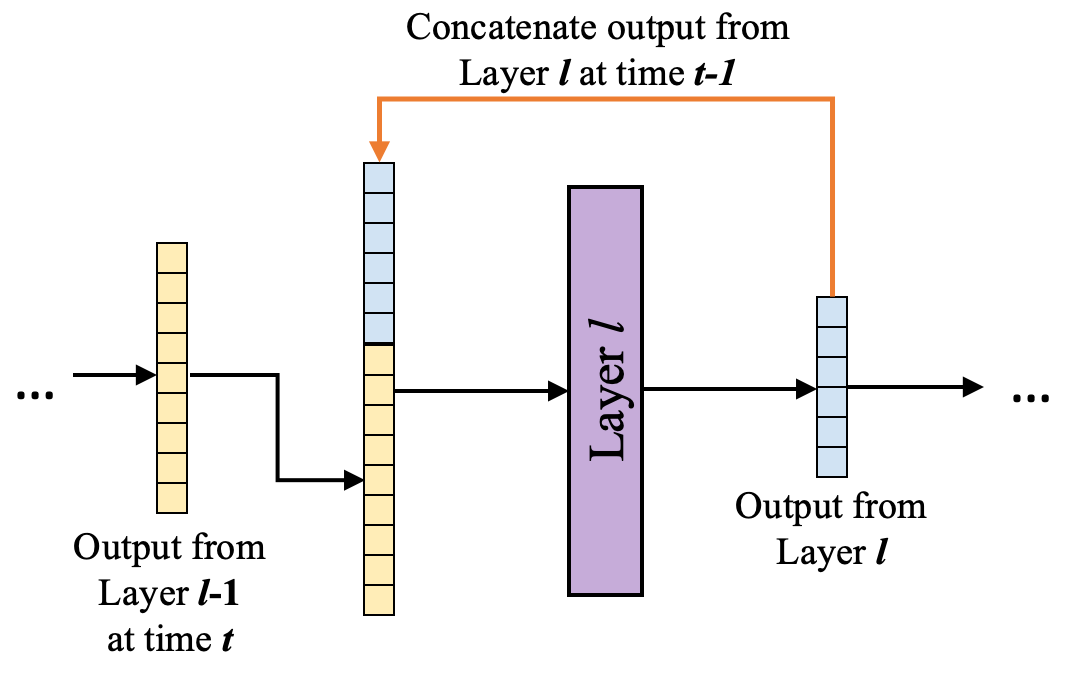
\includegraphics[width=0.89\textwidth]{lateral_concat}
    \caption[Lateral connections by concatenating the layer's output with the layer's input]{The lateral connections can be implemented by concatenating the layer's output at the previous time-step with the layer's input at the current time-step.}
    \figlbl{lateral_concat}
\end{figure}


Another option is to multiply the lateral input with an additional weight matrix and to add the result to the input. Therefore, \eqref{vso_1} is extended as follows:

\begin{align}\eqlbl{vso_13}
		\boldsymbol{a}^{[l]}[t] =  \boldsymbol{W}_x^{[l]} \cdot \boldsymbol{a}^{[l-1]}[t] + \boldsymbol{b}^{[l]} + \overbrace{\boldsymbol{W}_h^{[l]} \cdot \boldsymbol{a}^{[l]}[t-1] }^{\text{lateral connection}}
\end{align}

whereby $\boldsymbol{W}_x^{[l]}$ is the weight multiplied with the layer input and $\boldsymbol{W}_h^{[l]}$ the weight multiplied with the previous layer output. In both cases, the layer receives information about the activations at the previous timestep.
However, intuitively, recurrent connections seem only helpful if the model input is not static. Therefore, the model input is available over several timesteps and is optionally augmented after each step. Thus, the model receives different views of the same image and can adjust its activations if necessary. The following image augmentation techniques are applied:

\begin{itemize}
	\item \textbf{Color Jitter}: Randomly change the brightness, contrast, and saturation of the image.
	\item \textbf{Gaussian Blur}: Blur the image with randomly chosen Gaussian blur.
	\item \textbf{Random Rotation}: Randomly rotate the image with an angle in the range $[-15°, ..., 15°]$
	\item \textbf{Adjust Sharpness}: Randomly adjust the sharpness of the image.
\end{itemize}

These types of augmentation have proven successful in supervised image classification and are therefore expected to be helpful during lateral support as well.
Unlike image classification, however, the augmentation hyperparameters are initialised randomly and then kept fixed. This ensures that the model receives the same type of augmented view at each timestep and can thus learn to extract better representations from multiple well-known points of view\sidenote{for image classification, the augmentation hyperparameters are typically chosen randomly at each augmentation step to improve robustness}. 
\figref{mnist_augmented} visualises how this augmentation affects samples of the MNIST dataset \cite{Lecun_Bottou_Bengio_Haffner_1998}. The original image is shown on the left, and $9$ augmented versions of it are shown on the right.

\begin{figure}[h]
    \centering
    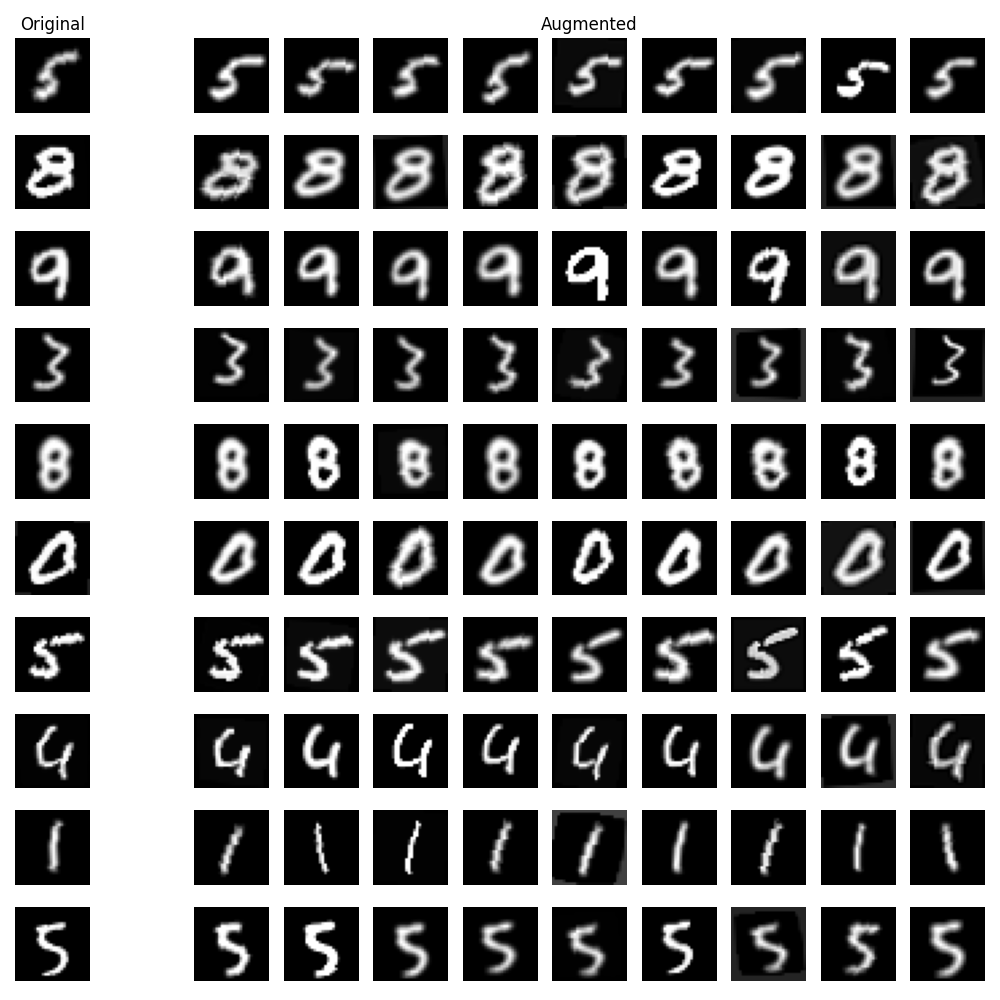
\includegraphics[width=0.99\textwidth]{mnist_augmented}
    \caption[Data augmentation applied on $10$ samples of the MNIST dataset]{Data augmentation applied on $10$ samples of the MNIST dataset. The original samples from the dataset are shown on the left, and $9$ augmented versions of the same samples are shown on the right.}
    \figlbl{mnist_augmented}
\end{figure}


Recurrent connections are typically used to process sequential data or text. Thereby, the data is usually first read token by token before an output is generated.\sidenote{for example, in text classification, all word tokens of a sentence are typically read before the model classifies a sentence. This is necessary because all information is required, and classification cannot be done on the basis of a single token.} Thus, such models depend on sequential timesteps and are typically trained with backpropagation through time (BTT). Thereby, the gradients flow backwards over several timesteps. This leads to well-known problems such as vanishing and exploding gradients.

In this thesis, BTT is not used, which means that a prediction is made after each timestep, but the prediction potentially improves with more timesteps. This leads to desirable properties: (i) Problems with vanishing or exploding gradients do not exist, regardless of how many timesteps the model requires. (ii) After each timestep, representations can be extracted according to \secref{horizontal_self_org_representations}. If an object representation can be assigned to one class label with a high probability, the sequential processing of different image views can be aborted. If this is not the case, further timesteps can be carried out until the model has sufficiently high confidence in its prediction. Thus, the number of timesteps can be sample-dependent.



\section{Results}\seclbl{horizontal_self_org_methods_results}
The results obtained by this model are presented in the following. It is important to note that these models aim not to achieve the best possible results in terms of classification accuracy on a benchmark. In large-scale comparisons, it has often been found that end-to-end backpropagation of error is far superior to other methods, especially in image classification \sidecite{Bartunov_Santoro_Richards_Marris_Hinton_Lillicrap_2018}. Instead, the aim is to examine interesting concepts that might lead to new learning principles.

\subsection{Dataset}\seclbl{horizontal_self_org_methods_dataset}
The model is trained and evaluated on the MNIST \cite{Lecun_Bottou_Bengio_Haffner_1998} dataset. MNIST is a dataset of handwritten digits with $60'000$ training samples and $10'000$ test samples.
In this thesis, the pre-defined training and test split is used.
The samples are images of a digit with the resolution $28 \times 28$ pixel in grayscale, i.e. has one colour channel.

In addition, the models are evaluated on MNIST-C \sidecite{Mu_Gilmer_2019}, a corrupted MNIST benchmark for testing the out-of-distribution robustness of image classification models. This dataset consists of the MNIST data with $15$ types of corruptions applied to the samples.

\subsection{Baseline Model}
The baseline model consists of $4$ fully connected layers with $512$, $256$, $128$ and $64$ neurons as shown in \figref{horizontal_org_arch1}.
No lateral connections or communication across multiple timesteps are used to train the baseline.
This model achieves an accuracy of $82.8\%$ on MNIST, and $64.7\%$ on MNIST-C.
This accuracy is relatively low compared to models trained with end-to-end backpropagation of error (c.f. \secref{hso_results_backprop}). 
This weak performance on classification is due to several reasons: First, the model is not explicitly trained for classification, e.g. with a cross-entropy loss. Instead, average image representations are extracted after training and used as object prototypes.
Furthermore, the goal of the model is to demonstrate novel concepts, and the hyperparameters are not optimised for a specific task like classification.

However, the model also has some very desirable properties; it is trained extremely fast because the local updates without propagating over layers are suitable for batch-gradient descent and not only mini-batch gradient descent.
Furthermore, each layer has a different accuracy in the range of $76.1\% - 81.9\%$. Due to the implicit voting by using the sum over the cosine similarities, the prediction of the entire model is better than that of a single layer.
The use of more layers (arranged sequentially or in parallel) would lead to even more votes and could, at best, further improve the result.



\subsection{Lateral Connections}
\begin{figure}[h]
    \centering
    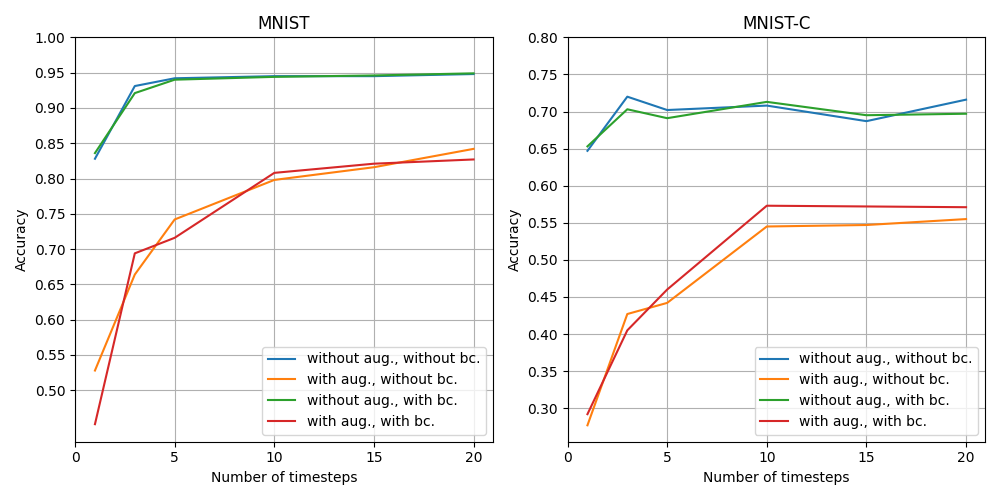
\includegraphics[width=0.99\textwidth]{hso_accuracy}
    \caption[Accuracy of models with lateral connection]{Accuracy of models with lateral connection on the MNIST and MNIST-C datasets for a different number of timesteps. The models are trained with and without data augmentation (aug.) as well as with and without backward connections (bc.).}
    \figlbl{digit_4_versions}
\end{figure}

In the human brain, lateral connections provide mutual support between neurons. In horizontal self-organisation, lateral connections are interpreted as recurrent connections within a layer. In this way, activations can be supported or corrected over several timesteps.
In \secref{horizontal_self_org_lateral_connections}, two suggestions are made on how lateral connections can be implemented; either the output of the layer is concatenated with the input of the layer, or an additional weight matrix is applied to the output of the layer and the result of this linear transformation is added to the input of the layer.
Both methods work well, but concatenation has, on average, resulted in $1.7$ p.p. better classification accuracy and is therefore preferred and used in the following. One disadvantage of concatenation is that the model has more parameters to train than if the weight matrix is split into two small matrices, as is the case for the second variant.
However, since the model is rather small, having a better classification performance is preferred over having less parameters.


The model is evaluated for $1$, $3$, $5$, $10$, $15$ and $20$ timesteps. Data augmentation is applied optionally after each timestep. In addition, backward connections are examined: With backward connections, the input of layer $l$ consists not only of the output of layers $l-1$ and $l$ (lateral connection) but also of the output of layer $l+1$. The intuition is that this implementation allows information to flow backwards. This could be helpful since the backward flow of information is not given without end-to-end backpropagation.

The results are shown in \figref{digit_4_versions}. It can be observed that data augmentation does not improve the results but worsens them (red and orange lines represent models with data augmentation, green and blue lines represent models without data augmentation). So the intuition that multiple views of the same image lead to a better prediction does not hold. Analysis shows that changing the input over timesteps leads to oscillations in the activations and, thus, to less stable results. An intuition is that without BTT, the model does not learn to leverage information from previous activations. When backpropagation through time is performed, the result is significantly better and comparable to that without data augmentation. This suggests that the model can learn to transmit information across timesteps with BTT but not without. However, not uing BTT is desirable as the updates remain local\sidenote{otherwise, they depend on the timestep}. It is also found that backward connections do not affect the result and thus do not improve the model.


Training over multiple timesteps without augmentation, on the other hand, seems very helpful: Static input over multiple timesteps improves the accuracy of the basline model on MNIST from $82.8\%$ (1 timestep) up to $94.8\%$ (20 timesteps). On MNIST-C, accuracy also improves significantly from $64.7\%$ to $71.6\%$.
 Thus, lateral connections with timesteps are helpful even if the input is static. However, an accuracy of $94.5\%$ is already obtained with $10$ timesteps, and, therefore, $10$ timesteps seem to be a good compromise between performance and computational efficiency. Also on MNIST-C the difference is marginal; with 10 timesteps the accuracy is $70.8\%$. Overall, lateral connections are an effective measure to improve the proposed model and it increases the model's accuracy by up to $12$ p.p.


\subsection{More Prototypes}
\begin{figure}[h]
    \centering
    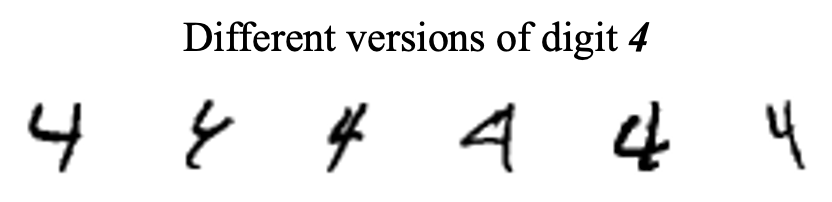
\includegraphics[width=0.49\textwidth]{digit_4_versions}
    \caption[Different versions of the digit ``$4$'' in the MNIST dataset]{Different versions of the digit ``$4$'' in the MNIST dataset.}
    \figlbl{digit_4_versions}
\end{figure}

For classification, a sample is compared to the average activation of each class. This average activation can be understood as an object prototype within a world model. Thus, it is compared to which prototype a sample fits best. The problem is that a single object prototype is not sufficient. As an example, \figref{digit_4_versions} shows different versions of the digit $4$ that can be found in the MNIST dataset. This demonstrates that a digit can be written in different ways\sidenote{this applies to all kinds of datasets: Most objects can have various visual characteristics (size, colour, shape) or look different from different viewpoints}.
Consequently, the digits and, thus, the activations look different for samples from the same class, and the use of more than one prototype per class is helpful. This is also in line with the human brain: The brain stores different views from the same object in its memory.

Therefore, instead of calculating the average activation per class, the activations per class are clustered for each layer using the k-means algorithm.
Afterwards, the average activation per cluster is calculated to obtain multiple prototypes per class and layer. For each class, the prototype that has the highest cosine similarity with the sample is selected and used for the voting. \figref{hso_accuracy_prototypes} shows the result.

\begin{figure}[h]
    \centering
    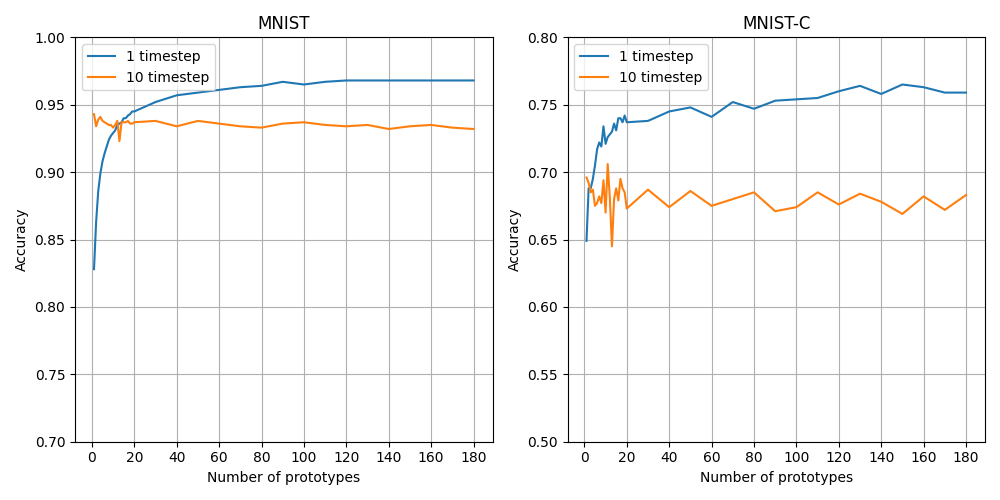
\includegraphics[width=0.99\textwidth]{hso_accuracy_prototypes}
    \caption[Accuracy of models with different number of prototypes]{Accuracy of models on MNIST and MNIST-C datasets using a different number of prototypes. One model is trained with $1$ timestep, the other model with $10$ timesteps.}
    \figlbl{hso_accuracy_prototypes}
\end{figure}

The use of more prototypes leads to significantly better results. For example, using $120$ prototypes per class improves the accuracy of the basline model on the MNIST dataset from $82.8\%$ to $96.8\%$ and on the MNIST-C dataset from $64.7\%$ to $76.4\%$.
This indicates the efficiency of using more prototypes.

Interestingly, using more prototypes only helps the model without timesteps. The model with more timesteps cannot benefit and the performance remains about the same with more prototypes. Despite extensive analysis, it remains unclear why the model with multiple timesteps does not benefit from multiple prototypes. One assumption is that multiple timesteps already separate the classes well and that further prototypes are not helpful.


\subsection{Comparison Backpropagation}\seclbl{hso_results_backprop}
To evaluate the performance of horizontal self-organisation, a model similar to the baseline model is trained with end-to-end backpropagation of the error. This model has an additional classification head with $10$ neurons, i.e. is a fully connected network with $512$, $256$, $128$, $64$ and $10$ neurons. The last layer with $10$ neurons is the classification head using a softmax activation to predict the classes. 
In addition, the batch size is reduced to $256$ samples since this model has no local updates and thus requires more memory. The other hyperparameters remain identical to the baseline model. The model with end-to-end backpropagation achieves an accuracy of $98.2\%$ on MNIST and $87.7\%$ on MNIST-C. In \tabref{vso_model_performance}, a comparison of the aforementioned models is given. There, it can be seen that the model with end-to-end backpropagation of error is superior for classification compared to the models trained with proxy objective functions. This is in line with \sideciteay{Bartunov_Santoro_Richards_Marris_Hinton_Lillicrap_2018}.



\begin{table}[h] 
    \centering
	 \begin{tabular}{l c c}
    	 & \textbf{Accuracy} & \textbf{Accuracy}\\
    	 \textbf{Model} & \textbf{MNIST} & \textbf{MNIST-C}\\
        \hline
		End-to-end backpropagation of error & $98.2\%$ & $87.7\%$\\
		Baseline & $82.8\%$ & $64.7\%$\\
		Baseline + $10$ timesteps & $94.5\%$ & $70.8\%$\\
		Baseline + $20$ timesteps & $94.8\%$ & $71.6\%$\\
		Baseline + $10$ prototypes & $92.9\%$ & $72.1\%$\\
		Baseline + $120$ prototypes & $96.8\%$ & $76.4\%$\\
		Baseline + $10$ timesteps + $120$ prototypes & $93.4\%$ & $67.6\%$\\
    \end{tabular}
    \caption[Accuracy of different models on MNIST and MNIST-C]{Accuracy of different models on MNIST and MNIST-C. The models are trained with a different number of timesteps and/or a different number of prototypes.}
    \tablbl{vso_model_performance}
\end{table}

However, the performance of the models based on horizontal self-organisation is only marginal worse; for example, the accuracy of the best model based on horizontal self-organisation is 1.4 p.p. worse  on MNIST compared to the model trained with end-to-end backpropagation of error. For MNIST-C, however, the difference is more significant. This could be due to how the classification is done: In the model based on end-to-end backpropagation, the activations within the network converge to $10$ neurons, using the most active neuron as the predicted class. Noise in the data is implicitly reduced during the forward pass\sidenote{as unimportant information is constantly removed until only class information is left}.
In contrast, the model based on horizontal self-organisation considers all activations for prediction, including those triggered by noise. Thus, the noise influences the prediction a lot. Alternative strategies for extracting the activations could provide a remedy: For example, a classification head could be applied to each layer to extract more robust representations and to filter out noise.